\part{Méthodologie}

  \section{Principe général}

    \begin{itemize}
      \item Génération des jeux de données
      \item Appel des fonctions à mesurer et stockage des résultats dans des Hashmaps % à détaiiler
      \item Tracé des graphiques
    \end{itemize}

  \section{Génération de données d'entrée de longueur variable}

    La génération est effectuée une seule fois par la méthode \texttt{generateRandomDatasets} de la classe
    \texttt{ComplexityMeasurements}.
    Ces jeux de données sont stockés sous forme d'un tableau à deux dimensions, qui est un attribut privé de la
     classe ComplexityMeasurements.

     Notre objectif est de travailler avec le même jeu de donnée pour chacun des algorithmes
     sur lesquels nous souhaitons effectuer des mesures de complexité temporelle.
   Afin de ne pas altérer le jeu de données initial, la classe \texttt{ArrayUtils} est instanciée pour chacun de ces algorithmes,
   et le jeu de données de test est cloné à chaque instanciation, puis passé en argument au constructeur de
   cette classe.

  \section{Mesure de la complexité temporelle}

    Pour mesurer la complexité temporelle, la classe \texttt{TimerUtils} sert à gérer le chronométrage de l'exécution d'une
    fonction. Elle permet de mémoriser le temps CPU du thread au sein lequel le programme s'exécute, et de récupérer
    la différence entre l'appel à \texttt{startTimer} et l'appel à \texttt{stopTimer}, via un appel à
    \texttt{getDuration}.

  \section{Utilisation des références de fonction}

    Pour appeler les fonctions que nous souhaitons mettre à l'épreuve sur notre jeu de données sans répéter le code
    servant à créer la HashMap qui stockera les résultats des mesures, une fonctionnalité de Java 8 est utilisée :
     il s'agit de la classe Consumer, qui permet de passer à une fonction dédiée à la mesure une référence
     vers une autre fonction, qu'elle se chargera d'appeller.

  \section{Tracé de graphiques}

    Pour tracer des graphiques, la bibliothèque JFreeChart est utilisée. Une classe a été développée pour s'interfacer
    avec cette bibliothèque de manière plus légère, dans la mesure où les configurations sont assez redondantes entre tous
    les graphiques qui doivent être tracés. Cette classe permet de tracer, dans une nouvelle fenêtre, les graphiques
    correspondant aux valeurs contenues dans une HashMap, grâce à sa méthode \texttt{drawHashmap}, ou de tracer sur
    un même graphe les données contenues dans plusieurs HashMaps grâce à sa méthode \texttt{addHashmapToDataset}, qui permet
     d'ajouter une nouvelle série de valeurs au graphique en cours de construction.


  \section{Un premier exemple : la recherche du minimum d'un tableau}

    Pour éprouver notre architecture, nous lançons notre programme sur la fonction servant à trouver la valeur
    minimale contenue dans un tableau. Cette méthode est ArrayUtils::findMin. Elle effectue une unique itération
    sur le tableau, quelle que soit la position de la valeur minimale. Sa complexité temporelle théorique
    est donc linéaire dans tous les cas, c'est-à-dire de la forme $\mathcal{O}(n)$.

    La courbe obtenue pour la mesure expérimentale de sa complexité temporelle est conforme à ce résultat théorique :
    elle nous montre effectivement une série de points apparentée à une fonction linéaire.

  \begin{center}
    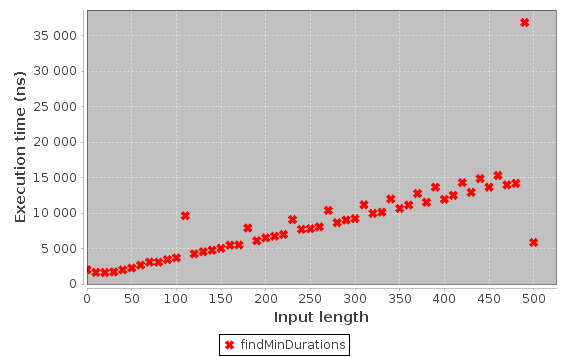
\includegraphics[width=13cm]{findMinTimeComplexity}
  \end{center}

